\section{Semut Adaptive Architecture}
\label{sec:architecture}

The Semut Adaptive Architecture models intelligent systems as a continuous interaction between reasoning, execution, and adaptive memory. Rather than treating retrieval systems, workflow engines, and feedback mechanisms as independent subsystems, the proposed architecture organizes them around three complementary memory structures: Artifact Memory, Action Graph, and Feedback Memory.

Figure~\ref{fig:architecture} conceptually illustrates the architecture.

The reasoning engine receives a user request together with context retrieved from the three memory structures. Based on the retrieved information, the reasoning engine determines one or more executable actions. Following execution, observations are recorded as feedback and incorporated back into the adaptive memory. This continuous update process allows future decisions to benefit from accumulated experience.

Unlike architectures that tightly couple memory with a specific reasoning algorithm, the proposed architecture separates adaptive memory from reasoning. Consequently, the reasoning engine may consist of a rule-based system, a Large Language Model, a future learning algorithm, or a human operator. Regardless of the implementation, all reasoning engines interact with the same adaptive memory interface.

The architecture consists of three primary components.

\subsection{Artifact Memory}

Artifact Memory stores persistent contextual information that may be retrieved during reasoning. Artifacts include both human-generated and machine-generated information such as documents, conversations, source code, structured databases, images, configuration files, and application state.

Unlike conventional storage systems that simply preserve information, Artifact Memory serves as contextual evidence for future reasoning. Retrieval mechanisms may employ semantic search, structured queries, metadata filtering, or other application-specific techniques depending on the underlying implementation.

\subsection{Action Graph}

The Action Graph represents executable behavior as a dynamic network of actions and observed transitions. Relationships between actions may evolve as additional executions, feedback, or coordination strategies are accumulated. Nodes correspond to executable operations, while edges describe ordering constraints, dependencies, alternative execution paths, or observed transitions.

Rather than representing only predefined workflows, the Action Graph evolves over time as new actions are executed and additional relationships are observed. Historical execution patterns provide valuable context for selecting future actions and coordinating complex tasks across heterogeneous software environments.

\subsection{Feedback Memory}

Feedback Memory records observations generated during or after execution. Feedback may originate from human evaluations, software systems, environmental sensors, execution metrics, or application-specific performance indicators.

Unlike traditional logging systems, Feedback Memory is intended to influence future reasoning directly. Successful outcomes strengthen confidence in previously executed actions, while failures, corrections, and human preferences become persistent knowledge that guides subsequent decisions.

\subsection{Interaction Between Memory Structures}

Although each memory structure serves a distinct purpose, they continuously influence one another. Retrieved artifacts provide context for selecting executable actions. Executed actions generate new artifacts and operational history. Feedback evaluates both retrieved information and executed behavior, allowing the adaptive memory to evolve through continual interaction.

The proposed architecture therefore treats artifacts, actions, and feedback as complementary representations of system experience rather than independent software components. This unified representation provides a common adaptive substrate upon which diverse reasoning engines may operate.

\begin{figure}[htbp]
    \centering
    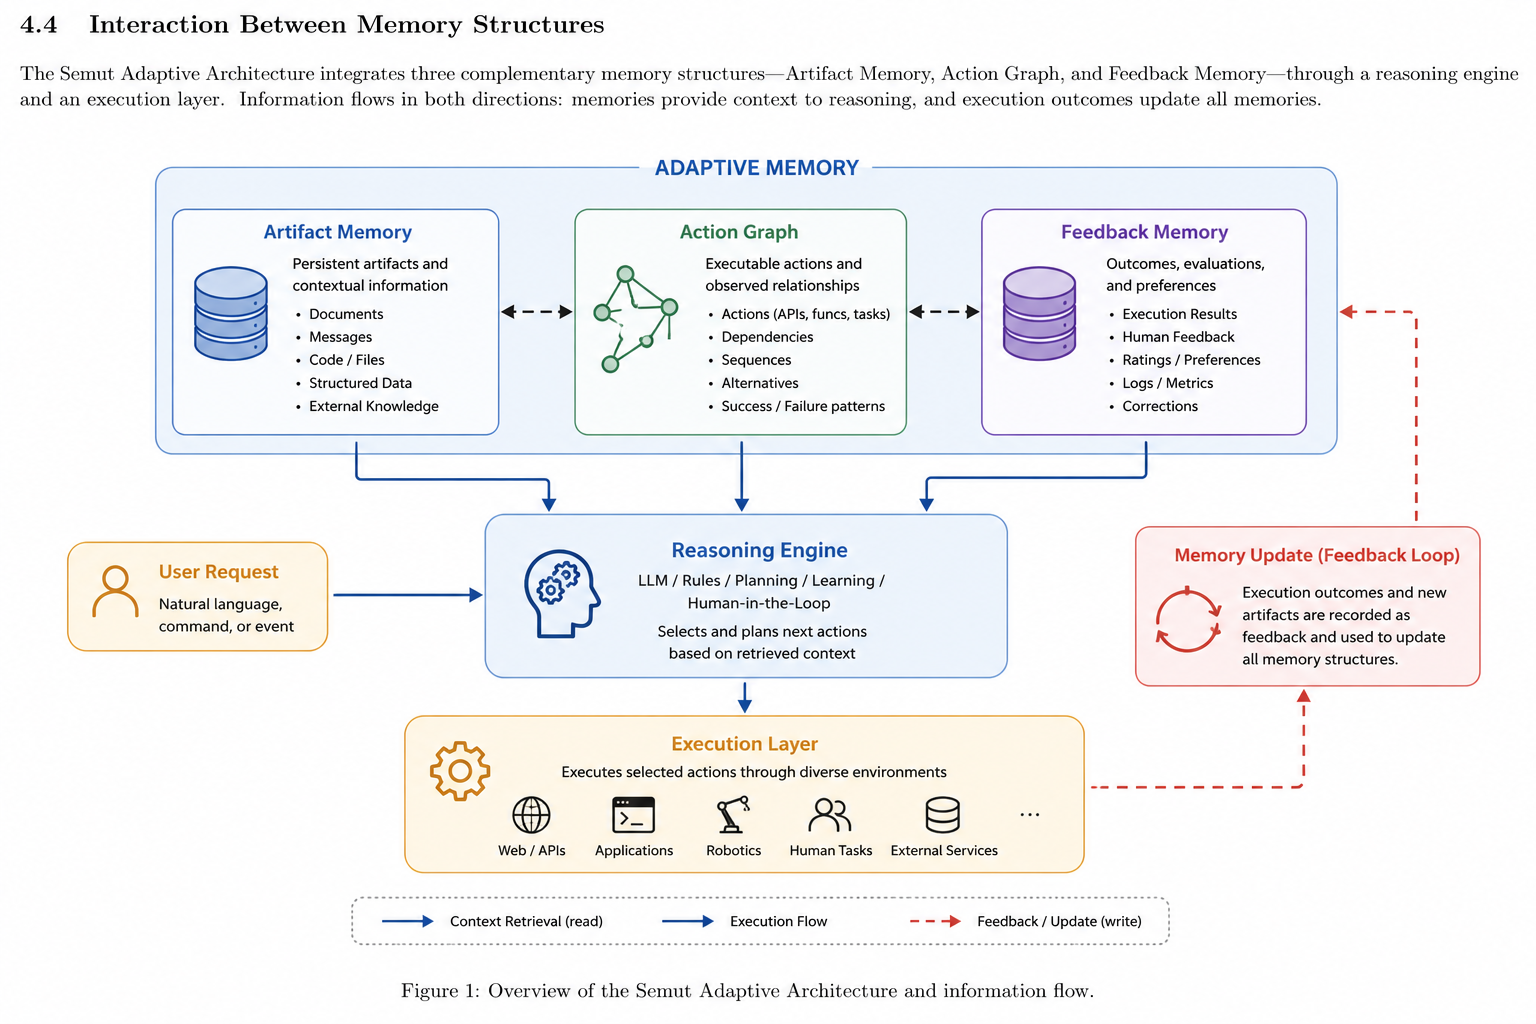
\includegraphics[width=\linewidth]{figures/architecture.PNG}
    \caption{Overview of the Semut Adaptive Architecture. Artifact Memory, Action Graph, and Feedback Memory provide contextual information to the reasoning engine. Execution outcomes update the adaptive memory, forming a continuous adaptive feedback loop.}
    \label{fig:architecture}
\end{figure}
